
 \chapter{Les broches d'interruptions}

 \index{Interruptions (broches)}
 Dans certains cas, il est souhaitable de récupérer la valeur d'une broche à tout moment du programme, même quand celui ci est occupé dans une tâche et même dans une fonction de temporisation \footnote{Voir delay(), delayMicroseconds()}. \\
 
 Pour remédier à ce problème, on peut utiliser les \colors{blue}{broches d'interruption} qui permettent de récupérer la main sur l'ensemble du programme lorsque'un évènement survient sur une broche.\\
 
 Concrètement, lorsque un évènement  \bold{e} survient sur la broche \bold{b}, la fonction \bold{f} est appelée, quelque soit l'état du programme principal. \\
 
 Prenons le cas d'un bouton qui doit changer l'état d'une LED à n'importe quel moment du programme.
 
 
\begin{Cpp}
 
     int ledPin = 13;    //Led interne
     int BOUTON = 2;  //Bouton relié à la broche 2 avec une résistance de charge
     
     volatile int state = LOW;  //Etat courant de la LED
     
     void setup() {
       
       Serial.begin(9600);//Vitesse de communication à 9600 bit/s
       
       pinMode(ledPin, OUTPUT);                //Led mise en sortie
       pinMode(BOUTON, INPUT_PULLUP);    //Bouton mis en entrée
       
       attachInterrupt(digitalPinToInterrupt(BOUTON), onEvent, CHANGE);  //Appel de la fonction onEvent à chaque changement de front du bouton
       Serial.println("Init");
     }
     
     void loop() {
       
      delay(5000); //Pause du programme principal
       
     }
     
     void onEvent() {
       
       state = !state; //Inverse l'état de la LED
       
       if(state){
         Serial.println("ON");
       }else{
         Serial.println("OFF");
       }
        digitalWrite(ledPin, state); //Met à jour l'état de la LED
     }
     
\end{Cpp}
 
 
 Ici, quelque soit l'action effectuée dans la fonction loop, dès qu'un front montant est détecté sur la broche BOUTON (2), la fonction onEvent() sera exécutée et changera l'état de la LED à chaque front.
 
 
 
 \subsection{Mode d'interruption}
 
 Il existe différents modes pour les broches :
 
 \begin{items}{blue}{\Bullet}
     \item RISING: front montant
     \item FALLING: Front descendant
     \item CHANGE: Front montant et descendant
 \end{items}
 
 \subsection{Chronogrammes d'interruption}
 
 
 \begin{numeric}{Exemple avec mode RISING}
     BOUTON & LLLLLLLHLLLLLLLLLL \\
     loop &  7D{EXECUTION} 6D{PAUSE} 7D{REPRISE} \\
     onEvent & 7D{INACTIVE} 6D{\bold{EXECUTION}} 7D{INACTIVE} \\
 \end{numeric}
 
 
 \begin{numeric}{Exemple avec mode FALLING}
     BOUTON & LLLLLLLHLLLLLLLLLL \\
     loop &  8D{EXECUTION} 6D{PAUSE} 6D{REPRISE} \\
     onEvent & 8D{INACTIVE} 6D{\bold{APPEL}} 6D{INACTIVE} \\
     \end{numeric}
 
 
 
 \begin{numeric}{Exemple avec mode CHANGE}
     BOUTON & LLLLLLLHHHHHHHHHHHHHHLLLLLLLLLLLLLL \\
     loop &  7D{EXECUTION} 8D{PAUSE} 6D{REPRISE} 8D{PAUSE} 6D{REPRISE}  \\
     onEvent & 7D{INACTIVE} 8D{\bold{EXECUTION}} 6D{INACTIVE} 8D{\bold{EXECUTION}} 6D{INACTIVE}\\
     \end{numeric}
 

     Par exemple, on souhaite réagir prioritairement à un capteur PIR quel que soit l'état du programme.


     \subsection{Exemple avec les capteur PIR}
     
     Les capteurs \glossary{PIR} (Passive-Infra-Red) détectent les rayonnements infrarouges émis par un objet.\\
     Puisque tout objet émet un rayonnement infrarouge, le capteur PIR est muni de deux cellules sensibles aux infrarouges qui vont détecter ces rayons infrarouges réfléchit ou émit par l'objet. \\
     
     Lorsqu’il n’y a pas de mouvement, le niveau d’infrarouge reçu est le même pour les deux cellules. 
     Lors du passage d’un objet, l’émission de ces rayons va être modifiée sur une cellule puis sur l’autre ce qui va permettre de détecter le mouvement. \\
     
     Le cache blanc, qui couvre et protège généralement le capteur, est une lentille de Fresnel avec plusieurs facettes qui permet de concentrer le rayonnement infrarouge sur les cellules.
     
     \subsection{Utilisation}
     
     Ces capteurs possèdent une broche de sortie qui est mise à l'état HAUT pendent une certaine durée
     \footnote{Cette durée est réglable avec le potentiomètre sur le capteur} lorsqu'il y a détection d'un mouvement.\\
     
     
     \begin{numeric}{Diagramme temporel du capteur}
         Présence & [green] LLLLLLHHHHHHHLLLLLLHHHLLLLLLLLLLLLHHHHHHLLLLL \\
         OUT & [blue] LLLLLLLHHHHHHHHLLLLLHHHHHHHHLLLLLLLHHHHHHHHLL \\
     \end{numeric}
     
     
\subsection{Code sans interruption}

Voici un code d'exemple pour réagir dès qu'une présence est détectée.

\begin{Cpp}{Code sans interruption}

#define LED 13    //Broche de la LED
#define OUT 2     //Broche du capteur PIR
    
void setup() 
{
      
  pinMode(LED, OUTPUT); //LED en sortie
  pinMode(OUT, INPUT);  //Broche du capteur en entrée
  Serial.begin(9600);   //Vitesse de communication à 9600 bauds

}//End setup
    
void loop(){
    
  outValue = digitalRead(OUT);          //Lire létat du capteur
        
    if (outValue == HIGH)                 //Détection d'un mouvement
    {
        Serial.println("Detection");
    }//End else
}//End loop
\end{Cpp}


Maintenant, supposons que la carte exécute un programme qui prend plusieurs secondes. Comment faire ?\\

On peut utiliser une interruption externe

\begin{Cpp}{Code avec interruption}
 

    #define LED 13    //Broche de la LED
    #define OUT 2     //Broche du capteur PIR
       
    void setup() {
      
      Serial.begin(9600);//Vitesse de communication à 9600 bit/s
      
      pinMode(LED, OUTPUT); //LED en sortie
      pinMode(OUT, INPUT);  //Broche du capteur en entrée
      
      attachInterrupt(digitalPinToInterrupt(OUT), presence, RISING);  //Appel de la fonction presence à chaque changement de front du bouton
      Serial.println("Init");
    }
    
    void loop() {
      
     delay(5000); //Pause du programme principal
      
    }
    
    void presence() {
      
      Serial.println("Presence !");
    }
    
\end{Cpp}



%\addPartText{Les modules de communication sans fil}
\part{Les modules de communication}



\chapter{Principes et théorie}
\section{Objectifs}

Ce chapitre a pour but de faire un petit tour d'horizon des différents modules de communication et les technologies associées.


\section{Les différents modules}

Il existe une multitude de modules: 


\begin{items}{blue}{\Circle}

    \item Modules Infrarouge
    \item Modules Radio basses fréquence (433MHz) 
    \item Modules Radio hautes fréquences (Wifi, Bluetooth) à 2.4 GHz

\end{items}

Les deux derniers modules se déclinent en une multitude de modules : 

\begin{items}{blue}{\Circle}

    \item Modules Lora
    \item Modules Xbee
    \item Modules HC-04 ou HC-05\footnote{Les modules HC-05 sont configurables en mode maître ou esclave et les modules HC-06 en 
    mode esclave uniquement.}
    \item Modules Crius
\end{items}


\section{Les modules Bluetooth}


\img{\rootImages/hc06.jpg}{Un module Bluetooth}{0.5}

La plupart des modules Bluetooth communiquent en liaison série (broche RX et TX) et se configurent avec les commandes AT.

\subsection{Configuration}

Il s'agit d'un jeu d'instruction pour gérer les paramètres des modules comme l'identifiant, le nom, la vitesse de communication, etc.\\

Ces commandes étaient utilisée à l'origine pour les modem Hayes Smartmodem 300 et sont donc également appelées \bold{commandes Hayes}.\\

Chaque commande est envoyée sous la forme d'une ligne de texte encodée en ASCII, débutant par le mot \bold{AT} et se terminant par le caractère \r seul (code ASCII 13).\\ 
Le module retourne une réponse sous la forme d'une ou plusieurs lignes selon la commande envoyée, chaque ligne se terminant par les caractères \r suivi de \n (codes ASCII 13 et 10).


\subsection{Branchements}

\img{\rootImages/arduino_hc_06.png}{Branchements du module Bluetooth}{0.3}

Pour l'exemple, nous nous baserons sur un module HC-06 ou HC-05.\\

il faut relier le « +5V » du module au  5 Volts de la carte Arduino et la masse du module à celle de la carte.\\
Ensuite, nous allons relier la broche TX du module à la broche 12 de la carte et la broche RX à la broche 10. \\


\subsection{Code Arduino}

\messageBox{Point-clé}{orange}{white}{Afin de lire les données du module, nous allons "émuler" une voie série, en l’occurrence les broches 3 et 2. C'est-à-dire que nous allons déclarer que ces broches recevront et enverront des données.}{white}


Pour cela, il faut utiliser la bibliothèque \bold{SoftwareSerial}.
Dans le logiciel Arduino, allez dans \bold{croquis} puis \bold{inclure une bibliothèque}  et sélectionnez \bold{SotfwareSerial}.

\img{\rootImages/software.png}{Inclusion de la bibliothèque SoftwareSerial}{0.7}

Maintenant, nous allons définir les broches du module : :

\begin{Cpp}{Définitions des broches RX et TX}
const int RX = 3; //RX du module
const int TX = 2;
\end{Cpp}

Après ceci, il faut déclarer un objet \bold{SoftwareSerial}  qui prendra en argument respectivement les broches TX et Rx, un peu comme lors de la déclaration d'un écran LCD (« LiquidCrystal lcd (RS,E,D4,D5,D6,D7); »).

On obtient donc :

\begin{Cpp}{Définition de l'objet SoftwareSerial}
#include <SoftwareSerial.h>

const int RX = 3; //RX du module
const int TX = 2;

SoftwareSerial device(RX,TX);
\end{Cpp}

Bien entendu, "device" peut être remplacé par ce que vous voulez. \\
Ensuite, on déclare que la communication carte-module peut débuter  avec "device.begin(9600) ;"
Où 115200 correspond à la vitesse de transmission en bauds (comme "Serial.begin(9600);") ;

\begin{Cpp}{Vitesse de communication}
SoftwareSerial device(RX,TX);
void setup() {
    device.begin(9600);
}
\end{Cpp}

\messageBox{Remarque importante}{red}{white}{Par la suite, en cas d'erreurs de transmission Bluetooth (pas de données...), il conviendra de vérifier le branchement des broches RX et TX (essayer de les intervertir) et d'éventuellement changer la vitesse de communication  car certains modules communiquent à 115200 bauds !}{white}

Pour lire les données du module, ce sont les mêmes fonctions que pour le port série : \\
En effet : \\

Pour le port série :	\\	

\begin{items}{blue}{\Triangle}
    \item Serial,begin(115200);
    \item Serial.available();
    \item Serial.read();	
    \item Serial.print();
    \item Serial.println();
\end{items}

Pour le module Bluetooth : \\

\begin{items}{blue}{\Triangle}
    \item crius.begin(115200);
    \item device.available();
    \item device.read();	
    \item device.print();
    \item device.println();
\end{items}


Tant que des données (caractères) sont disponibles, nous allons les assembler en une chaîne de caractère (concaténation). \\
Ensuite, avec un \bold{if}, nous allons voir si cette chaîne en question correspond par exemple à "a". \\ 

Il faut donc définir un caractère x et une chaîne de caractère.\\
Donc dans le programme Arduino, avant la fonction \bold{setup}, on rajoute :

\begin{Cpp}{Définition des structures du message}
#include <SoftwareSerial.h>

const int RX = 3; //RX du module
const int TX = 2;

char c;
String message;

\end{Cpp}

La boucle while va permettre de lire les données : 
Dans la boucle \bold{loop} : on écrit :

\begin{Cpp}{Boucle de lecture partielle}
 void loop() {
 
    while() {
    
    }//Fin while

 }//Fin void loop

\end{Cpp}

Maintenant que la boucle va attendre des données, il suffit de les lire et de les transformer en chaîne de caractère. \\
Pour cela : \\

\begin{items}{blue}{\Triangle}
    \item on lit le premier caractère c
    \item on définit que la chaîne message = message + c 
\end{items}
On obtient :

\begin{Cpp}{Boucle de lecture complète}
 void loop() {
 
    while(device.available()>0) {
    
        c = device.read();
        message = message + c;
    }//Fin while

 }//Fin void loop

\end{Cpp}

La structure conditionnelle est très simple : \\
Après la boucle « while », mettez : \\

\begin{Cpp}{Structure conditionnelle}
 void loop() {
 
    while(device.available()>0) {
    
        c = device.read();
        message = message + c;
    }//Fin while
    
    if(message=="c") {
    
        Serial.println("C);
    }//Fin if message=="c"

 }//Fin void loop

\end{Cpp}

\section{Les modules radio }

\img{\rootImages/radio.jpg}{Un module receveur et émetteur}{0.5}

\subsection{Choix de l'antenne}

La plupart du temps, on utilise une antenne \bold{quart d'onde} ou \bold{demi-onde}.\\
La fréquence vaut :

$$ \lambda = \frac{c}{\nu}$$
 avec $\lambda$ la longueur d'onde en mètre, $c$ la vitesse de l'onde en $m\cdot s^-1 $ et  $\nu $ la fréquence de l'onde en Hz

 D'ou : 

 $$ \lambda = \frac{3\cdot 10^{8}}{433\cdot 10^{6}} = 0.69 ~m $$

 Or on prend une antenne valant le quart du résultat, c'est à dire 17 cm.

 \subsection{Branchements}

 \subsubsection{Module émetteur}
 \begin{items}{blue}{\Bullet}
    \item \inputPin{VCC} sur le \outputPin{+5V} de l'Arduino
    \item \inputPin{GND} sur le \outputPin{GND} de l'Arduino
    \item \inputPin{Data} sur la broche \outputPin{D12} de l'Arduino
 \end{items}

 \subsubsection{Module receveur}

 \begin{items}{blue}{\Bullet}
    \item \inputPin{VCC} sur le \outputPin{+5V} de l'Arduino
    \item \inputPin{GND} sur le \outputPin{GND} de l'Arduino
    \item \inputPin{Data} sur la broche \outputPin{D11} de l'Arduino
 \end{items}


 \section{Les modules Xbee }

 \img{\rootImages/xbee.png}{Un module Xbee}{0.5}

 Ce module communique via une liaison série.\\ L'un des inconvénient de ce module est l'espacement des broches de 2mm et non de 2.54 mm.
 Il faut donc utiliser un shield adapté.

 La fréquence de communication est cette fois ci de 2.4GHz.


 \chapter{Introduction au projet MySensors}


\section{Présentation}

Ce chapitre a pour but d'introduire la mise en place d'une passerelle et d'une sonde MySensors dans un projet de domotique

\subsection{Organigramme}

\begin{figure}[h]
  \centering
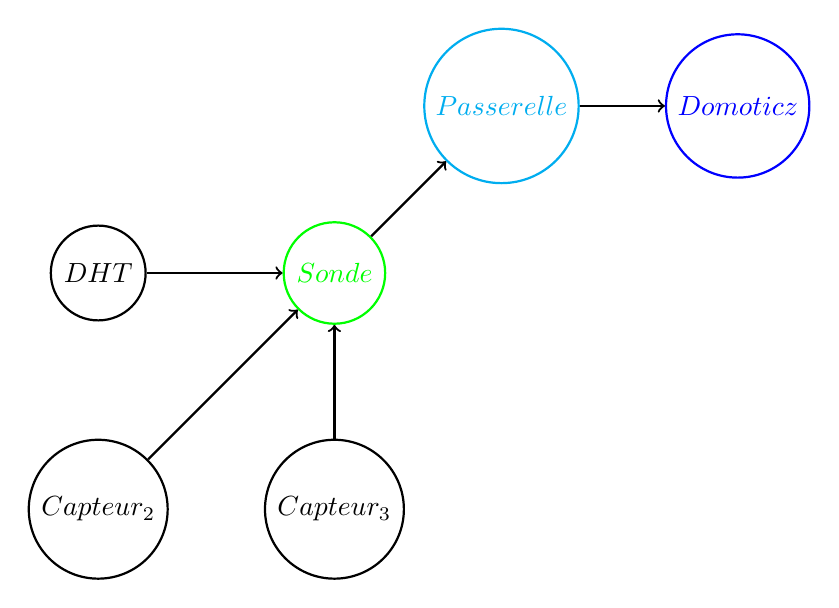
\begin{tikzpicture}[node distance={30mm}, thick, main/.style = {draw, circle}]
  \node[main] (1) [color=green] {$Sonde$}; 
  \node[main] (2) [above right of=1, color=cyan] {$Passerelle$}; 
  \node[main] (3) [left of=1] {$DHT$}; 
  \node[main] (4) [below of=3] {$Capteur_2$}; 
  \node[main] (5) [below of=1] {$Capteur_3$}; 
  \node[main] (6) [right of=2, color=blue] {$Domoticz$};
  
  \draw[->] (3) -- (1);
  \draw[->] (4) -- (1);
  \draw[->] (5) -- (1);

  \draw[->] (1) -- (2);
  \draw[->] (2) -- (6);
\end{tikzpicture} 
\caption{Les différents composants du projet}
\end{figure}

  \subsection{Principe}

  Les capteurs vont être analysés par la sonde MySensors.\\
  Cette dernière enverra à distance les informations vers la passerelle qui se chargera d'envoyer les informations au serveur Domoticz via une liaison USB.\\


  Une sonde représente un endroit physique, un lieu de mesure. \\
  Si vous souhaitez par la suite faire d'autres relevés dans un endroit différent, il suffira d'ajouter une sonde et de garder la passerelle.\\
  Chaque sonde est caractérisée par un identifiant de noeud (NODE\_ID) et chaque capteur possède un identifiant enfant sur la sonde qui lui est rattachée (CHILD\_ID)
  \begin{figure}[h]
    \centering
  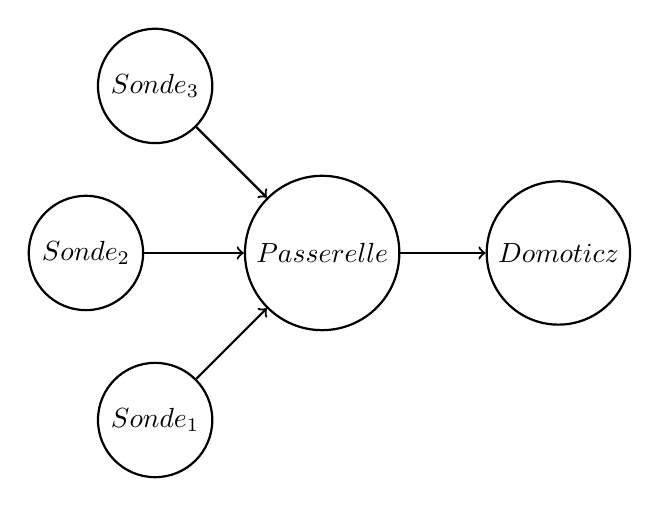
\begin{tikzpicture}[node distance={30mm}, thick, main/.style = {draw, circle}]
    \node[main] (1) {$Passerelle$}; 
    \node[main] (2) [below left of=1] {$Sonde_1$}; 
    \node[main] (3) [left of=1] {$Sonde_2$}; 
    \node[main] (4) [above left of=1] {$Sonde_3$}; 

    \node[main] (5) [right of=1] {$Domoticz$};
    
    \draw[->] (2) -- (1);
    \draw[->] (3) -- (1);
    \draw[->] (4) -- (1);
  
    \draw[->] (1) -- (5);
    \end{tikzpicture} 
    \caption{Une extension possible}
  \end{figure}



  \section{Présentation de la passerelle}

  \img{\rootImages/pin.png}{Circuit imprimé vu de dessus, coté composants}{0.5}\label{TEST}

  \img{\rootImages/side.png}{Vue de coté}{0.4}
  \img{\rootImages/passerelle_emetteur.png}{Vue de la passerelle et de l'émetteur}{0.4}
  \img{\rootImages/dessus.png}{Vue de dessus}{0.4}


  \section{Présentation de la sonde}

  \img{\rootImages/pcb.png}{Circuit imprimé vu de dessus, coté composants}{0.5}\label{TEST}


  \img{\rootImages/s4.jpg}{Sonde vue de dessus sans la nappe}{0.25}
  \img{\rootImages/s3.jpg}{Sonde vue de dessus avec la nappe}{0.25}
  
  
  
\chapter{Configuration de Domoticz}

Une fois que la passerelle est fonctionnelle, nous allons configurer Domoticz pour que la plateforme reçoive les données en provenance de la passerelle.

\section{Ajout de la passerelle}

Tout d'abord, allez dans la section \bold{Configuration > Matériel}

\img{\rootImages/hardware.png}{Emplacement du matériel}{0.5}

Ensuite, saisissez les informations suivantes :

\img{\rootImages/add_gateway.png}{Paramétrage de la passerelle}{0.5}

Le port série sélectionné sera celui où est raccordé la passerelle en liaison USB.
Il ne faut pas prendre les noms simplifiés des ports USB (\italic{COM\_XXX}) mais le nom le plus complet.\\
Pour plus de simplicité, veuillez déconnectez tous les autres périphériques du Raspberry-Pi\\.


S'il s'agit d'un autre capteur (température...) il suffit de parcourir la liste pour le trouver?


\section{Recherche des capteurs}

Visualisons les données en provenance de la sonde en allant dans \\
\bold{Configuration > Matériel}\\.

L'ensemble de vos dispositif apparaît. En cas de liste trop longue, saisissez \bold{Gateway} dans la barre de recherche.


\img{\rootImages/search.png}{Recherche de la passerelle}{0.5}


\messageBox{Remarque}{orange}{white}{Si le dispositif n'apparaît pas immédiatement, patientez quelques instants.}{black}

\img{\rootImages/gateway.png}{La passerelle est détectée}{0.4}



Pour visualisez les valeurs des capteurs, il faut sélectionner la passerelle avec l'ID de la sonde (ici, 30).

\img{\rootImages/nodes.png}{Sélection de la passerelle}{0.5}

En cliquant dessus, on voit que la partie \bold{Enfants} est mise à jour et contient les 3 capteurs avec les ID définis dans le programme de la sonde (31,32 et 33 en ce qui me concerne)

\img{\rootImages/enfants.png}{Visualisation des enfants}{0.4}


\section{Visualisation des données}

Maintenant que nous savons que la sonde envoi les bonnes données, nous allons ajouter les capteurs dans les dispositifs.
Pour cela, allez dans \bold{Configuration > Dispositifs}, les 3 capteurs de la sonde (Tension batterie, humidité et température) apparaissent dans la liste.\\
Si vous ne les trouvez pas, vous pouvez nettoyer la page des capteurs en sélectionnant les capteurs non-utilisés et en le mettant à la poubelle.

\img{\rootImages/disp.png}{Visualisation des capteurs}{0.25}

Les capteurs apparaissent sous les 3 noms suivants : 

\img{\rootImages/names.png}{Nom des capteurs}{0.6}

Pour ajouter un dispositif, il suffit de cliquer sur la flèche verte et de choisir le nom du dispositif.

\img{\rootImages/fleche.png}{Ajout des dispositifs}{0.5}

\img{\rootImages/voltage.png}{Ajout des dispositifs - Sélection du nom}{0.5}

Il suffit de cliquer dans le menu \bold{Mesures}

\img{\rootImages/mesure.png}{Mesures}{0.4}

Et apparaît la tension de la batterie.

\img{\rootImages/volt.png}{tension de la batterie}{0.5}

On procède de même pour l'humidité et la température, les dispositifs seront mis dans l'onglet  \bold{Température}.

\img{\rootImages/temp.png}{Mesures de l'humidité et de la température}{0.4}


Pour visualiser les données, il suffit de cliquer sur le bouton \bold{logs}


\section{Conclusion}

Nous avons vu une utilisation de Domoticz via les sondes MySensors mais énormément de dispositifs domotiques existent sur Domoticz.


